This chapter aims to present the reader with useful explanations of the field-specific terms used in the dissertation as well as provide insight into the significant research previously carried out. This chapter aims to present a general idea of the existing research, both in the field of computing, and in the field of biology . Included are example of pre-existing applications, either implementing similar algorithms, or possessing a comparable purpose.

\section{Previous Work} \label{prevwork}
Evolutionary computing is the field of artificial intelligence devoted to solving problems by implementing Darwinian principles of evolution. It includes evolutionary algorithms, genetic algorithms, and genetic programming. Starting from the premise of a common biological ancestor, Darwin proposed evolution from the simple to the complex, given enough time. With mutations appearing in a creature's genetic code, he stipulated that beneficial mutations providing an advantage would be passed on to future generations \cite{darwinbook1859}. Accumulating multiple such mutations would lead to a completely new organism, different from the original.

\subsection{Evolutionary Algorithms}
Since initially proposed by Alan Turing in 1950 under the form of "learning machines" \cite{turing1950computing} akin to biological systems, such simulations became the study of subsequent decades. Selection, key to Darwinian principles, was first simulated by Alex Fraser, in 1957 \cite{fraser1960simulation}.

When faced with complex optimization problems, performing a linear search, especially through a large solution space usually associated with such problems, may prove ineffective. Evolutionary algorithms became regarded as a method of solving complex optimisation problems in the 1970s \cite{holland1975adaptation}. In general, several biological methods, such as sexual or asexual reproduction or genetic mutation, are used in order to evolve the population of a particular system with respect to a certain predetermined fitness function. As such, more ``fit" individuals have a higher chance of being selected to pass on their genome to the next generation, as seen in Figure~\ref{fig:evo}, thus increasing the fitness factor of the overall population after each iteration. Over a longer period of time spanning from a few thousand, to a million generations, the population will evolve towards a solution. This, however, suffers from diminishing returns \cite{fumagalli2015speed}, as the population tends to meet an impasse in locally optimal points, rather than reach the global maximum.

\begin{figure}[!th]
	\centering
	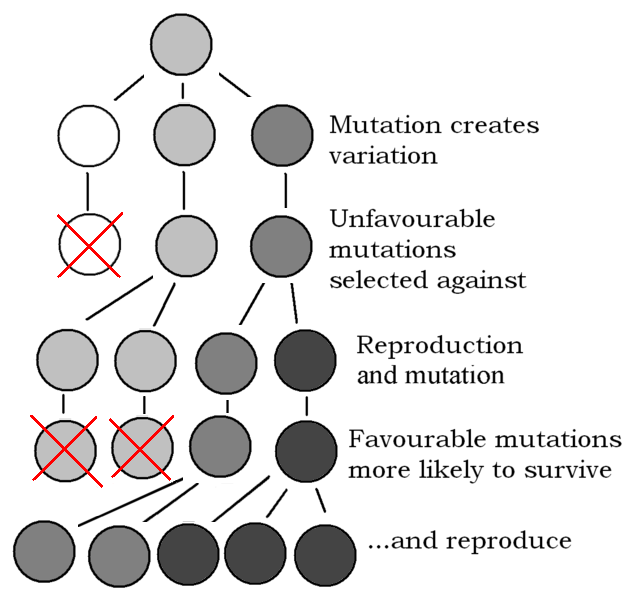
\includegraphics[scale=0.35]{images/evo}
	\caption{\label{fig:evo}A diagram showing a simplified process of natural selection.}
	\textit{Copyright Wikimedia Foundation, under Creative Commons Attribution-Share Alike~\cite{mutationandselection}}
\end{figure}

\subsection{Biological Simulation}
Building upon the basis of genetic algorithms, biological simulations become possible.

A more prominent paper in the field of artificial evolution is ``Evolving Virtual Creatures" by Karl Sims \cite{sims1994evolving}. The paper details an evolutionary system which focuses evolving a population of creatures consisting of three dimensional blocks with respect to various movement-specific tasks (such as walking, running, jumping, climbing, and swimming). An example of such creature is represented in Figure~\ref{fig:evc}. Noteworthy is the fact that both the creature's morphology and it's ``brain" are evolved.
\begin{figure}[!th]
	\centering
	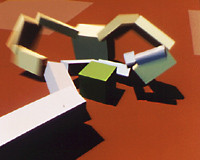
\includegraphics[scale=1]{images/crabvsarm}
	\caption{\label{fig:evc}A screenshot from the simulator build by Karl Sims ``Evolved Virtual Creatures"}
\end{figure}
While the initial randomly created generation was incapable of performing any task, subsequent generations showed significant improvement. Even after a relatively low number of generations, some creatures were becoming adapted to their environment. In the swimming example, some creatures were successful in developing fin-like appendages, used for locomotion, while other replicated the waving motion of water-snakes. The scope of the experiment, however is quite limited, as creatures are observed individually, with a rather basic fitness function, and not in competition with each other.

A more recent paper, Dan Lessin's et al. ``Open-ended behavioral complexity for evolved virtual creatures" \cite{lessin2013open}, deals with the open-ended nature of evolution, previously unexplored in Karl Sims's paper. The paper proposes the evolution of a creature's brains as well as body, thus allowing it to better adapt to its environment. While the evolution of the body is fairly similar to the method described by Karl Sims, the control part of a creature is evolved differently. This involves encapsulating a creature's previously learned skills. An example of such a creature, together with its subroutines can seen in Figure~\ref{fig:open}.
\begin{figure}[!th]
	\centering
	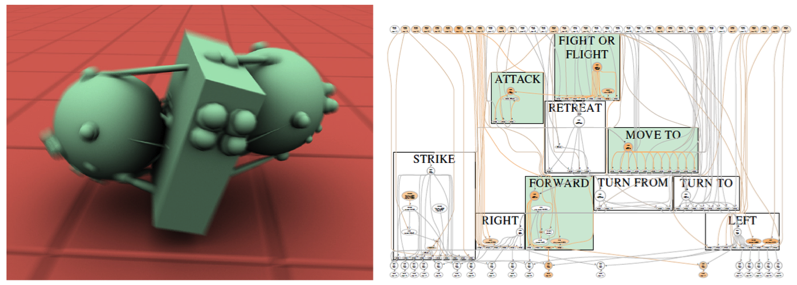
\includegraphics[scale=1]{images/cirtualcreatures}
	\caption{\label{fig:open}An example of a creature's physiognomy and control circuit}
\end{figure}
The benefits presented are persistent memory, allowing a creature to store a certain behaviour once it has been learned, and overall simplicity, allowing the whole procedure to be called as a single node, instead of actively recreating the movement. By allowing newer nodes to be modified more frequently than older ones, the algorithm simulates the forming of habits. By changing the fitness function, creatures can adapt to different environments, or learn more complex behaviours, without ``forgetting" their previous training. This, in turn, provides a more accurate representation of nature.

\subsection{Virtual Worlds}
While research in the field of Genetic Algorithms is extensive, it deals mostly either with problems of optimization, or with the best few individuals of a population. This is not the case when trying to simulate the entire population, as being the very best only gives a marginally higher chance of passing genes to the next generation. Simply being ``good enough" to eat sufficient food in order to be able to live and reproduce is adequate. This is especially important when dealing with a heterogeneous environment, where food density might vary. In this scenario, simply being in an area with more food could be considered more beneficial than becoming the best individual. A common occurrence in such simulations is the gathering of individuals around food clusters, with those to do so dying off.

\subsubsection{Darwinbots}

A similar application in appearance is Darwinbots \cite{darwinbots}. Darwinbots presents itself as an artificial life simulator, where creatures, called ``bots" can compete for food in a simulated two dimensional environment. The most successful ``bots" will live on to pass their genes to subsequent generations. Darwinbots, however, specialises in simulating Von Neumann machines.
\begin{figure}[!th]
	\centering
	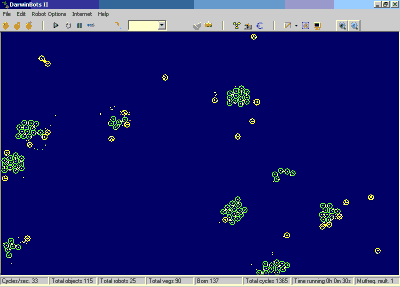
\includegraphics[scale=1]{images/darwinbots}
	\caption{A screenshot from a Darwinbots simulation}
\end{figure}

Darwinbots specialises in providing a platform for interactivity between multiple species of organisms with wildly varying behavioural patterns. Should it prove beneficial to do so, creatures may combine different purposes to form more complex, specialised, multi-cellular organisms, with constituent parts focusing independently on locomotion, sensory input, digestion, and combat.

The creatures implement a piece of code represented as a syntax tree as their inherent algorithm. Using tree cross-over operations described in ``A Field Guide to Genetic Programming" \cite{fieldguide}, these algorithms, which essentially form the control circuit of a particular individual, are evolved. Due to the nature of mutation in tree cross-over individuals of the same species can evolve in different directions, should both be more optimal than the current incarnation, due to divergent evolution.

\subsubsection{Goopies}

A more simple approach is taken by Paul T. Oliver in his project called ``Goopies" \cite{goopies}. The creatures live in a bounded, circular world, together with food pellets and obstacles. An example of such a world can be seen in Figure~\ref{fig:goop}. A creature's behaviour is determined by its intrinsic neural network. Creature physiognomy exists only for the purpose of conveying information about certain parameters of its control circuit. Unlike Darwinbots, at the end of one generation, the best individuals with respect to a fitness function are selected. Crossover is performed on their genes and a new population is created.

\begin{figure}[!th]
	\centering
	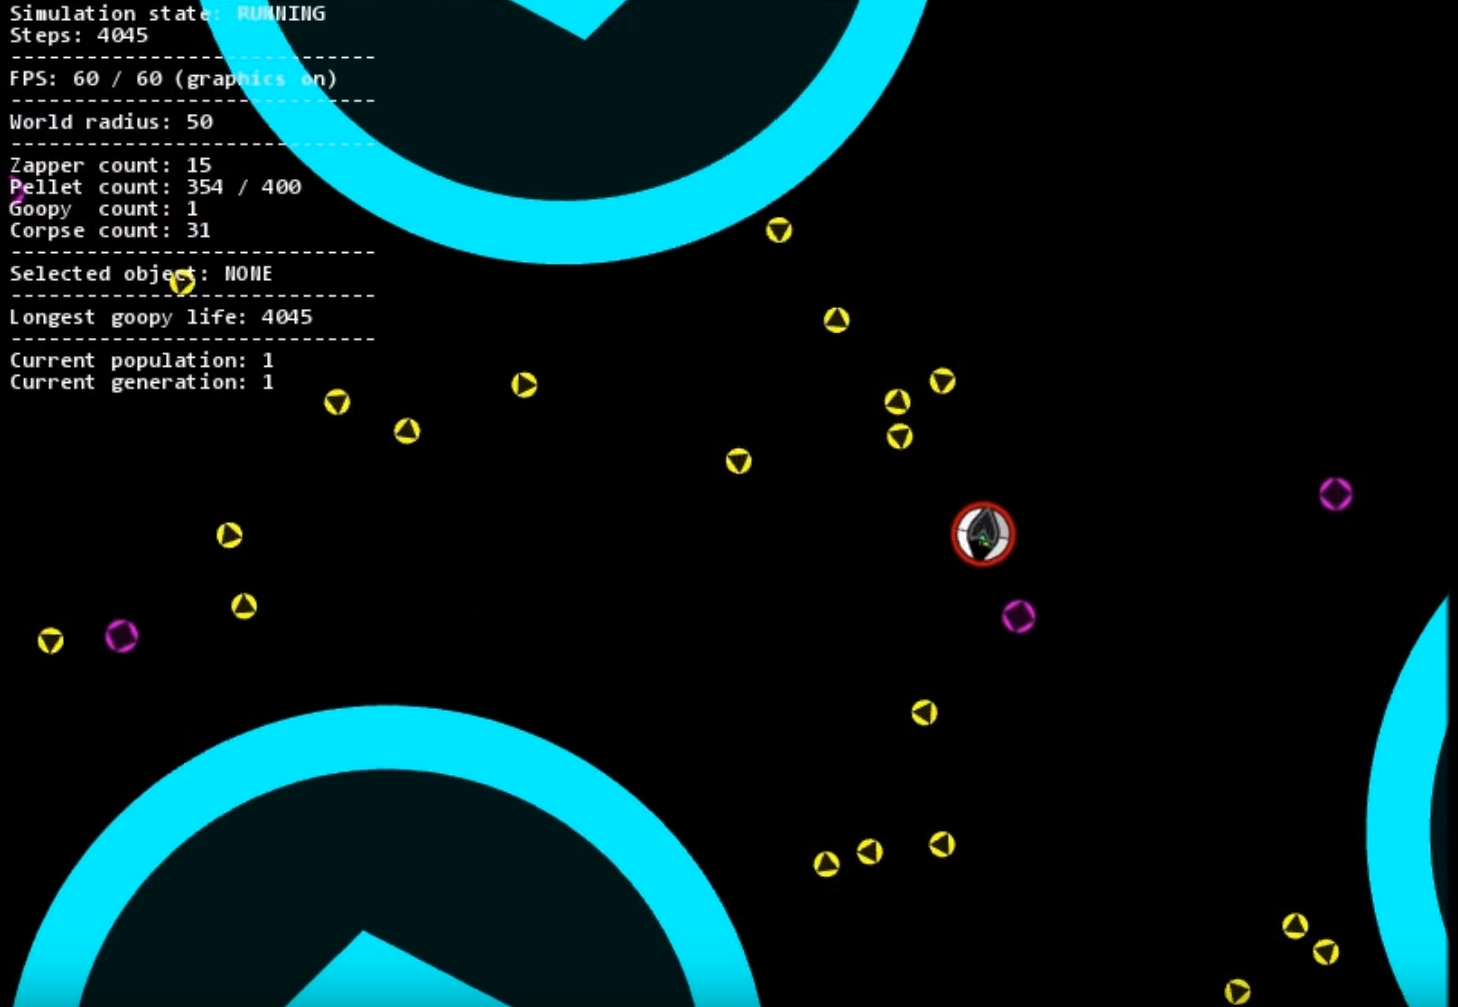
\includegraphics[scale=0.3]{images/guppies}
	\caption{\label{fig:goop}A ``goopie" searching for food}
\end{figure}

In this simulate world, creatures do not actively interact with each other like in Darwinbots. The impact made by an individual on the others is the food he consumes and his corpse. This has generated a peculiar behaviour where ``Goopies" would linger close to others close to their death, similar to carrion-eater behaviour in animals.


\subsubsection{Conway's Game of Life}
Introduced by John Conway in 1970 \cite{gardner1970mathematical}, the eponymous game is a two-dimensional implementation of a cellular automation. According to a predefined rule, the subsequent states are created from an initial state. Building on von Neumann ideas of a machine capable of self-replication, Conway attempted to simplify the concepts. Due to the fact that it implemented a universal Turing Machine \cite{igblan}, this sparked interest for the game since its inception.

\begin{figure}[!th]
	\centering
	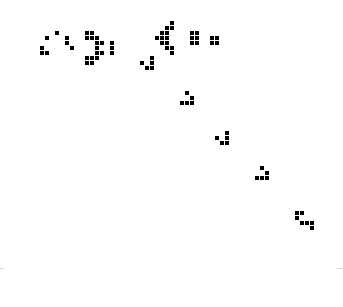
\includegraphics[scale=0.6]{images/glidergun}
	\caption{\label{fig:glider}A cellular formation that has the property to generate ``gliders"}
\end{figure}

It is particularly simple to observe patterns among the population. Notable among the categories of patterns are ``still lifes", ``oscillators", and ``spaceships". The first denote a series of arrangements of cells that, if left alone, do not change in any way \cite{griffeath2003new}. Oscillators are a set of repeating patterns, characterised by a period. ``Spaceships" are patterns that can translate themselves across the grid. Two gliders, seen in Figure~\ref{fig:glider}, can be shot at a particular angle at a static two-by-two block in order to move it. This can act as memory for a more complex system implementing a finite-state machine.

\section{Summary}
Presented above are different examples of evolutionary computing, ranging from genetic algorithms used for optimization problems, to entire simulated virtual worlds. The ``Blobs on a Plane" project is based on such algorithms, and in turn, attempts to provide a simplified simulation where population dynamics can be observed in relation to environmental parameters.
The next chapter will present the requirements for the project.